\documentclass[D:/studies/WinnerS/Erhebungen/IPhO1718/paper/problem_solving/main/TaylorFrancis/interactapasample]{subfiles}

%\usepackage{Sweave}

\begin{document}






\section{Results}

The primary interest is on Problem comprehension (PC). The correlations (Table \ref{correlation_table}) among the variables indicate that ability for problem comprehension and heuristic physics problem solving are significantly related to the highest round of the participants in the competition. The motivational scales, on the other hand, have no apparent relation to success in the physics Olympiad as measured through highest qualified round. Neither do the motivational measures relate to the other cognitive measures such as content knowledge and ability of problem conceptualization. Moreover, the sense of belonging tends to correlate negatively with the other variables.

\begin{sidewaystable}
\caption{Correlations among measured variables.}
\label{correlation_table}
% latex table generated in R 3.4.3 by xtable 1.8-2 package
% Wed Sep 26 19:40:11 2018
\begin{tabular}{lcccccccccc}
  \toprule
Measure & 1 & 2 & 3 & 4 & 5 & 6 & 7 & 8 & 9 & 10 \\ 
  \midrule
1 Heuristic physics problem solving & - & .27 & .29* & .33** & .32* & .03 & .03 & .26 & -.09 & .16 \\ 
  2 Problem comprehension &  & - & .32** & .41*** & .32* & .10 & .01 & .18 & .19 & .31** \\ 
  3 Achievement round 1 &  &  & - & .68*** & .33** & .000 & -.07 & .25 & .09 & .05 \\ 
  4 Highest round &  &  &  & - & .25 & .12 & -.01 & .29* & .12 & .08 \\ 
  5 Cog. abilities &  &  &  &  & - & -.02 & -.10 & .12 & .000 & .09 \\ 
  6 Self-efficacy physics &  &  &  &  &  & - & .42*** & .37*** & .28* & -.18 \\ 
  7 Sense of belonging &  &  &  &  &  &  & - & .34** & .29* & -.01 \\ 
  8 Expectancy physics competition &  &  &  &  &  &  &  & - & .21 & .04 \\ 
  9 Value physics competition &  &  &  &  &  &  &  &  & - & -.07 \\ 
  10 Age &  &  &  &  &  &  &  &  &  & - \\ 
   \bottomrule
\end{tabular}\end{sidewaystable}



\begin{figure}
\centering
\includegraphics[width=.6\textwidth]{D:/studies/WinnerS/Erhebungen/IPhO1718/paper/problem_solving/results/ordinal_regression/img/boxplot}
% % Created by tikzDevice version 0.11 on 2019-01-06 13:27:31
% !TEX encoding = UTF-8 Unicode
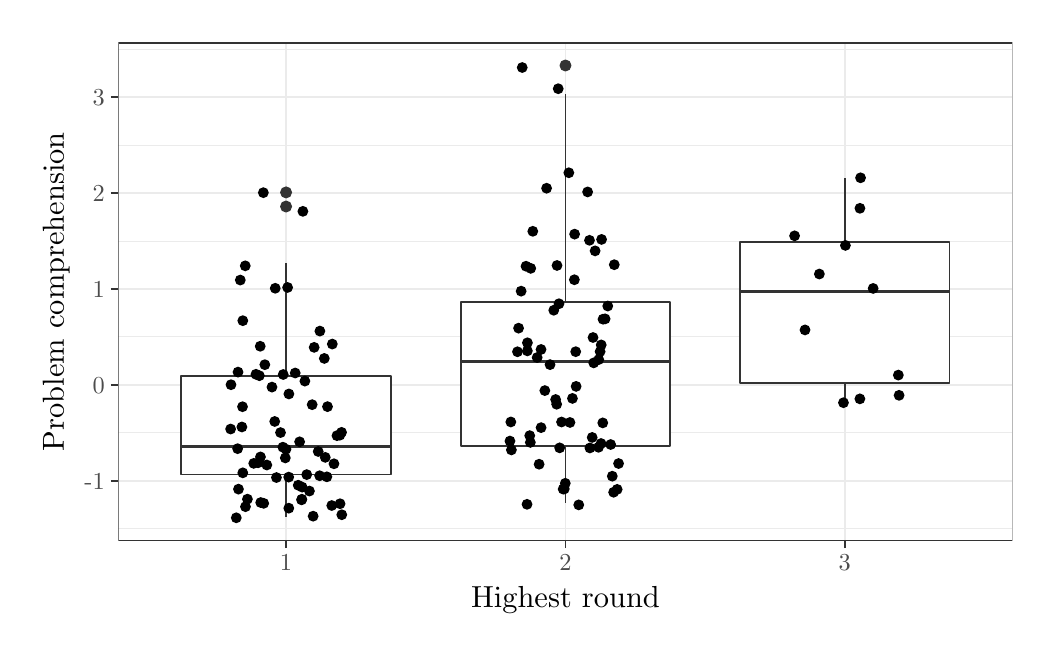
\begin{tikzpicture}[x=1pt,y=1pt]
\definecolor{fillColor}{RGB}{255,255,255}
\path[use as bounding box,fill=fillColor,fill opacity=0.00] (0,0) rectangle (361.35,216.81);
\begin{scope}
\path[clip] (  0.00,  0.00) rectangle (361.35,216.81);
\definecolor{drawColor}{RGB}{255,255,255}
\definecolor{fillColor}{RGB}{255,255,255}

\path[draw=drawColor,line width= 0.6pt,line join=round,line cap=round,fill=fillColor] (  0.00,  0.00) rectangle (361.35,216.81);
\end{scope}
\begin{scope}
\path[clip] ( 32.80, 31.53) rectangle (355.85,211.31);
\definecolor{fillColor}{RGB}{255,255,255}

\path[fill=fillColor] ( 32.80, 31.53) rectangle (355.85,211.31);
\definecolor{drawColor}{gray}{0.92}

\path[draw=drawColor,line width= 0.3pt,line join=round] ( 32.80, 35.77) --
	(355.85, 35.77);

\path[draw=drawColor,line width= 0.3pt,line join=round] ( 32.80, 70.42) --
	(355.85, 70.42);

\path[draw=drawColor,line width= 0.3pt,line join=round] ( 32.80,105.08) --
	(355.85,105.08);

\path[draw=drawColor,line width= 0.3pt,line join=round] ( 32.80,139.73) --
	(355.85,139.73);

\path[draw=drawColor,line width= 0.3pt,line join=round] ( 32.80,174.39) --
	(355.85,174.39);

\path[draw=drawColor,line width= 0.3pt,line join=round] ( 32.80,209.05) --
	(355.85,209.05);

\path[draw=drawColor,line width= 0.6pt,line join=round] ( 32.80, 53.10) --
	(355.85, 53.10);

\path[draw=drawColor,line width= 0.6pt,line join=round] ( 32.80, 87.75) --
	(355.85, 87.75);

\path[draw=drawColor,line width= 0.6pt,line join=round] ( 32.80,122.41) --
	(355.85,122.41);

\path[draw=drawColor,line width= 0.6pt,line join=round] ( 32.80,157.06) --
	(355.85,157.06);

\path[draw=drawColor,line width= 0.6pt,line join=round] ( 32.80,191.72) --
	(355.85,191.72);

\path[draw=drawColor,line width= 0.6pt,line join=round] ( 93.37, 31.53) --
	( 93.37,211.31);

\path[draw=drawColor,line width= 0.6pt,line join=round] (194.33, 31.53) --
	(194.33,211.31);

\path[draw=drawColor,line width= 0.6pt,line join=round] (295.28, 31.53) --
	(295.28,211.31);
\definecolor{drawColor}{gray}{0.20}
\definecolor{fillColor}{gray}{0.20}

\path[draw=drawColor,line width= 0.4pt,line join=round,line cap=round,fill=fillColor] ( 93.37,152.18) circle (  1.96);

\path[draw=drawColor,line width= 0.4pt,line join=round,line cap=round,fill=fillColor] ( 93.37,157.28) circle (  1.96);

\path[draw=drawColor,line width= 0.6pt,line join=round] ( 93.37, 91.04) -- ( 93.37,131.80);

\path[draw=drawColor,line width= 0.6pt,line join=round] ( 93.37, 55.37) -- ( 93.37, 40.09);
\definecolor{fillColor}{RGB}{255,255,255}

\path[draw=drawColor,line width= 0.6pt,line join=round,line cap=round,fill=fillColor] ( 55.52, 91.04) --
	( 55.52, 55.37) --
	(131.23, 55.37) --
	(131.23, 91.04) --
	( 55.52, 91.04) --
	cycle;

\path[draw=drawColor,line width= 1.1pt,line join=round] ( 55.52, 65.56) -- (131.23, 65.56);
\definecolor{fillColor}{gray}{0.20}

\path[draw=drawColor,line width= 0.4pt,line join=round,line cap=round,fill=fillColor] (194.33,203.14) circle (  1.96);

\path[draw=drawColor,line width= 0.6pt,line join=round] (194.33,117.79) -- (194.33,192.95);

\path[draw=drawColor,line width= 0.6pt,line join=round] (194.33, 65.56) -- (194.33, 45.18);
\definecolor{fillColor}{RGB}{255,255,255}

\path[draw=drawColor,line width= 0.6pt,line join=round,line cap=round,fill=fillColor] (156.47,117.79) --
	(156.47, 65.56) --
	(232.18, 65.56) --
	(232.18,117.79) --
	(156.47,117.79) --
	cycle;

\path[draw=drawColor,line width= 1.1pt,line join=round] (156.47, 96.13) -- (232.18, 96.13);

\path[draw=drawColor,line width= 0.6pt,line join=round] (295.28,139.45) -- (295.28,162.38);

\path[draw=drawColor,line width= 0.6pt,line join=round] (295.28, 88.49) -- (295.28, 80.85);

\path[draw=drawColor,line width= 0.6pt,line join=round,line cap=round,fill=fillColor] (257.42,139.45) --
	(257.42, 88.49) --
	(333.14, 88.49) --
	(333.14,139.45) --
	(257.42,139.45) --
	cycle;

\path[draw=drawColor,line width= 1.1pt,line join=round] (257.42,121.61) -- (333.14,121.61);
\definecolor{fillColor}{RGB}{0,0,0}

\path[fill=fillColor] (195.95, 74.15) circle (  1.96);

\path[fill=fillColor] (184.10, 97.61) circle (  1.96);

\path[fill=fillColor] ( 75.87, 64.68) circle (  1.96);

\path[fill=fillColor] (280.89,107.59) circle (  1.96);

\path[fill=fillColor] (300.96,162.56) circle (  1.96);

\path[fill=fillColor] (100.84, 55.31) circle (  1.96);

\path[fill=fillColor] ( 98.97, 46.19) circle (  1.96);

\path[fill=fillColor] (192.92, 74.32) circle (  1.96);

\path[fill=fillColor] ( 85.70, 95.03) circle (  1.96);

\path[fill=fillColor] (210.66, 66.18) circle (  1.96);

\path[fill=fillColor] (174.79, 64.24) circle (  1.96);

\path[fill=fillColor] (190.77, 82.45) circle (  1.96);

\path[fill=fillColor] ( 77.74,110.93) circle (  1.96);

\path[fill=fillColor] ( 83.28, 59.59) circle (  1.96);

\path[fill=fillColor] ( 89.89, 54.25) circle (  1.96);

\path[fill=fillColor] (208.65,111.58) circle (  1.96);

\path[fill=fillColor] (207.81, 74.00) circle (  1.96);

\path[fill=fillColor] (108.11, 54.51) circle (  1.96);

\path[fill=fillColor] (203.99, 68.74) circle (  1.96);

\path[fill=fillColor] ( 83.72, 91.05) circle (  1.96);

\path[fill=fillColor] (207.25,102.17) circle (  1.96);

\path[fill=fillColor] (206.27, 65.18) circle (  1.96);

\path[fill=fillColor] ( 97.76, 51.47) circle (  1.96);

\path[fill=fillColor] (294.78, 81.29) circle (  1.96);

\path[fill=fillColor] ( 81.69, 59.37) circle (  1.96);

\path[fill=fillColor] (192.23, 64.98) circle (  1.96);

\path[fill=fillColor] (204.29,104.85) circle (  1.96);

\path[fill=fillColor] ( 92.22, 65.22) circle (  1.96);

\path[fill=fillColor] ( 84.03,101.69) circle (  1.96);

\path[fill=fillColor] ( 77.73, 55.95) circle (  1.96);

\path[fill=fillColor] ( 99.45,150.44) circle (  1.96);

\path[fill=fillColor] (197.64,142.20) circle (  1.96);

\path[fill=fillColor] ( 79.40, 46.44) circle (  1.96);

\path[fill=fillColor] (207.38,140.29) circle (  1.96);

\path[fill=fillColor] ( 78.62,130.75) circle (  1.96);

\path[fill=fillColor] (186.88, 85.67) circle (  1.96);

\path[fill=fillColor] (211.73, 48.94) circle (  1.96);

\path[fill=fillColor] (197.55,125.72) circle (  1.96);

\path[fill=fillColor] ( 75.38, 39.70) circle (  1.96);

\path[fill=fillColor] (202.34,157.45) circle (  1.96);

\path[fill=fillColor] (203.16, 64.94) circle (  1.96);

\path[fill=fillColor] ( 96.67, 92.02) circle (  1.96);

\path[fill=fillColor] ( 94.33, 54.41) circle (  1.96);

\path[fill=fillColor] ( 73.47, 87.79) circle (  1.96);

\path[fill=fillColor] ( 93.10, 61.34) circle (  1.96);

\path[fill=fillColor] ( 78.70, 43.72) circle (  1.96);

\path[fill=fillColor] ( 77.41, 72.52) circle (  1.96);

\path[fill=fillColor] ( 92.34, 91.48) circle (  1.96);

\path[fill=fillColor] (104.98, 63.66) circle (  1.96);

\path[fill=fillColor] ( 85.16,157.19) circle (  1.96);

\path[fill=fillColor] (110.08,102.48) circle (  1.96);

\path[fill=fillColor] (277.12,141.59) circle (  1.96);

\path[fill=fillColor] (198.18, 87.19) circle (  1.96);

\path[fill=fillColor] (196.85, 82.84) circle (  1.96);

\path[fill=fillColor] ( 91.36, 70.50) circle (  1.96);

\path[fill=fillColor] (181.78,129.84) circle (  1.96);

\path[fill=fillColor] (195.55,164.38) circle (  1.96);

\path[fill=fillColor] ( 93.93,122.93) circle (  1.96);

\path[fill=fillColor] (180.08,130.61) circle (  1.96);

\path[fill=fillColor] (180.58,102.94) circle (  1.96);

\path[fill=fillColor] ( 94.36, 43.18) circle (  1.96);

\path[fill=fillColor] (174.27, 67.43) circle (  1.96);

\path[fill=fillColor] (300.72, 82.68) circle (  1.96);

\path[fill=fillColor] (110.68, 59.22) circle (  1.96);

\path[fill=fillColor] ( 99.08, 46.41) circle (  1.96);

\path[fill=fillColor] (193.50, 50.08) circle (  1.96);

\path[fill=fillColor] (191.28,130.88) circle (  1.96);

\path[fill=fillColor] (111.76, 69.38) circle (  1.96);

\path[fill=fillColor] ( 89.27, 74.51) circle (  1.96);

\path[fill=fillColor] (198.03, 99.73) circle (  1.96);

\path[fill=fillColor] (204.54, 95.69) circle (  1.96);

\path[fill=fillColor] ( 73.34, 71.78) circle (  1.96);

\path[fill=fillColor] (199.13, 44.37) circle (  1.96);

\path[fill=fillColor] ( 76.83,125.61) circle (  1.96);

\path[fill=fillColor] (113.50, 40.81) circle (  1.96);

\path[fill=fillColor] (101.81, 49.37) circle (  1.96);

\path[fill=fillColor] (206.85, 99.77) circle (  1.96);

\path[fill=fillColor] (206.35, 96.88) circle (  1.96);

\path[fill=fillColor] ( 82.49, 91.56) circle (  1.96);

\path[fill=fillColor] ( 76.17, 50.06) circle (  1.96);

\path[fill=fillColor] (112.81, 69.56) circle (  1.96);

\path[fill=fillColor] (107.19, 97.29) circle (  1.96);

\path[fill=fillColor] (191.15, 80.73) circle (  1.96);

\path[fill=fillColor] ( 93.35, 64.48) circle (  1.96);

\path[fill=fillColor] ( 77.63, 79.84) circle (  1.96);

\path[fill=fillColor] ( 76.01, 92.35) circle (  1.96);

\path[fill=fillColor] (193.90, 50.14) circle (  1.96);

\path[fill=fillColor] (113.42, 70.58) circle (  1.96);

\path[fill=fillColor] (174.59, 74.33) circle (  1.96);

\path[fill=fillColor] (191.71,194.75) circle (  1.96);

\path[fill=fillColor] ( 84.21, 45.22) circle (  1.96);

\path[fill=fillColor] (184.81, 59.06) circle (  1.96);

\path[fill=fillColor] ( 86.42, 58.78) circle (  1.96);

\path[fill=fillColor] (203.01,139.97) circle (  1.96);

\path[fill=fillColor] (300.73,151.54) circle (  1.96);

\path[fill=fillColor] ( 98.27, 67.16) circle (  1.96);

\path[fill=fillColor] ( 88.28, 86.93) circle (  1.96);

\path[fill=fillColor] ( 89.46,122.64) circle (  1.96);

\path[fill=fillColor] (182.53,143.23) circle (  1.96);

\path[fill=fillColor] (295.49,138.13) circle (  1.96);

\path[fill=fillColor] (181.64, 66.95) circle (  1.96);

\path[fill=fillColor] ( 94.39, 84.45) circle (  1.96);

\path[fill=fillColor] (181.42, 69.39) circle (  1.96);

\path[fill=fillColor] (103.15, 40.29) circle (  1.96);

\path[fill=fillColor] (176.99, 99.70) circle (  1.96);

\path[fill=fillColor] (305.51,122.58) circle (  1.96);

\path[fill=fillColor] ( 99.17, 50.80) circle (  1.96);

\path[fill=fillColor] (213.52, 59.31) circle (  1.96);

\path[fill=fillColor] ( 84.12, 61.70) circle (  1.96);

\path[fill=fillColor] (180.56,100.02) circle (  1.96);

\path[fill=fillColor] (286.07,127.79) circle (  1.96);

\path[fill=fillColor] (314.61, 91.27) circle (  1.96);

\path[fill=fillColor] (112.88, 44.78) circle (  1.96);

\path[fill=fillColor] (102.80, 80.58) circle (  1.96);

\path[fill=fillColor] (211.25, 54.74) circle (  1.96);

\path[fill=fillColor] (191.99,117.05) circle (  1.96);

\path[fill=fillColor] (103.52,101.29) circle (  1.96);

\path[fill=fillColor] (188.76, 95.05) circle (  1.96);

\path[fill=fillColor] (209.61,116.22) circle (  1.96);

\path[fill=fillColor] (185.50,100.53) circle (  1.96);

\path[fill=fillColor] (211.97,131.16) circle (  1.96);

\path[fill=fillColor] (187.51,158.79) circle (  1.96);

\path[fill=fillColor] (207.90,111.47) circle (  1.96);

\path[fill=fillColor] (213.01, 49.97) circle (  1.96);

\path[fill=fillColor] (194.27, 52.16) circle (  1.96);

\path[fill=fillColor] (185.52, 72.28) circle (  1.96);

\path[fill=fillColor] (190.10,114.70) circle (  1.96);

\path[fill=fillColor] (177.39,108.23) circle (  1.96);

\path[fill=fillColor] ( 85.29, 44.93) circle (  1.96);

\path[fill=fillColor] (105.59,107.17) circle (  1.96);

\path[fill=fillColor] (105.51, 54.90) circle (  1.96);

\path[fill=fillColor] (109.88, 44.14) circle (  1.96);

\path[fill=fillColor] (108.34, 79.87) circle (  1.96);

\path[fill=fillColor] (207.19, 66.54) circle (  1.96);

\path[fill=fillColor] (178.31,121.60) circle (  1.96);

\path[fill=fillColor] (205.04,136.15) circle (  1.96);

\path[fill=fillColor] (178.71,202.41) circle (  1.96);

\path[fill=fillColor] (107.53, 61.54) circle (  1.96);

\path[fill=fillColor] (100.17, 89.10) circle (  1.96);

\path[fill=fillColor] (180.44, 44.58) circle (  1.96);

\path[fill=fillColor] (314.88, 83.96) circle (  1.96);

\path[draw=drawColor,line width= 0.6pt,line join=round,line cap=round] ( 32.80, 31.53) rectangle (355.85,211.31);
\end{scope}
\begin{scope}
\path[clip] (  0.00,  0.00) rectangle (361.35,216.81);
\definecolor{drawColor}{gray}{0.30}

\node[text=drawColor,anchor=base east,inner sep=0pt, outer sep=0pt, scale=  0.88] at ( 27.85, 50.06) {-1};

\node[text=drawColor,anchor=base east,inner sep=0pt, outer sep=0pt, scale=  0.88] at ( 27.85, 84.72) {0};

\node[text=drawColor,anchor=base east,inner sep=0pt, outer sep=0pt, scale=  0.88] at ( 27.85,119.38) {1};

\node[text=drawColor,anchor=base east,inner sep=0pt, outer sep=0pt, scale=  0.88] at ( 27.85,154.03) {2};

\node[text=drawColor,anchor=base east,inner sep=0pt, outer sep=0pt, scale=  0.88] at ( 27.85,188.69) {3};
\end{scope}
\begin{scope}
\path[clip] (  0.00,  0.00) rectangle (361.35,216.81);
\definecolor{drawColor}{gray}{0.20}

\path[draw=drawColor,line width= 0.6pt,line join=round] ( 30.05, 53.10) --
	( 32.80, 53.10);

\path[draw=drawColor,line width= 0.6pt,line join=round] ( 30.05, 87.75) --
	( 32.80, 87.75);

\path[draw=drawColor,line width= 0.6pt,line join=round] ( 30.05,122.41) --
	( 32.80,122.41);

\path[draw=drawColor,line width= 0.6pt,line join=round] ( 30.05,157.06) --
	( 32.80,157.06);

\path[draw=drawColor,line width= 0.6pt,line join=round] ( 30.05,191.72) --
	( 32.80,191.72);
\end{scope}
\begin{scope}
\path[clip] (  0.00,  0.00) rectangle (361.35,216.81);
\definecolor{drawColor}{gray}{0.20}

\path[draw=drawColor,line width= 0.6pt,line join=round] ( 93.37, 28.78) --
	( 93.37, 31.53);

\path[draw=drawColor,line width= 0.6pt,line join=round] (194.33, 28.78) --
	(194.33, 31.53);

\path[draw=drawColor,line width= 0.6pt,line join=round] (295.28, 28.78) --
	(295.28, 31.53);
\end{scope}
\begin{scope}
\path[clip] (  0.00,  0.00) rectangle (361.35,216.81);
\definecolor{drawColor}{gray}{0.30}

\node[text=drawColor,anchor=base,inner sep=0pt, outer sep=0pt, scale=  0.88] at ( 93.37, 20.52) {1};

\node[text=drawColor,anchor=base,inner sep=0pt, outer sep=0pt, scale=  0.88] at (194.33, 20.52) {2};

\node[text=drawColor,anchor=base,inner sep=0pt, outer sep=0pt, scale=  0.88] at (295.28, 20.52) {3};
\end{scope}
\begin{scope}
\path[clip] (  0.00,  0.00) rectangle (361.35,216.81);
\definecolor{drawColor}{RGB}{0,0,0}

\node[text=drawColor,anchor=base,inner sep=0pt, outer sep=0pt, scale=  1.10] at (194.33,  7.44) {Highest round};
\end{scope}
\begin{scope}
\path[clip] (  0.00,  0.00) rectangle (361.35,216.81);
\definecolor{drawColor}{RGB}{0,0,0}

\node[text=drawColor,rotate= 90.00,anchor=base,inner sep=0pt, outer sep=0pt, scale=  1.10] at ( 13.08,121.42) {Problem comprehension};
\end{scope}
\end{tikzpicture}

\caption{Problem conceptualization scores over highest achieved round of participant.}
\label{problem_concept_skills}
\end{figure}




In order to estimate the effect of ability of problem conceptualization on success in the physics Olympiad (RQ 1), generalized linear models that account for the ordinal metric of the dependent variable are utilized. Furthermore, covariates that were established in previous research are included into the models in order to assess how stable the effects are. However, achievement in round 1 in the physics Olympiad was omitted as a covariate because of the high correlation with the other cognitive measures that were of more interest to us. We use proportional odds models in order to predict success in the physics Olympiad. 

The modelling assumptions of parallel slopes hold in our case, $\chi^2=0.04, p=.98$. The interesting parameters in the model are the effects (not the intercepts), which can be interpreted in accordance with the regression parameters in linear regression (B�rkner \& Vuorre, 2018). Table \ref{propOddModel} shows the results from the analysis. As can be expected, generic physics problem solving and physics problem conceptualization are significantly positively related with highest qualified round of the participants. The relationship holds when entering the predictors to the models. 

When analyzing the influence of the categories (concept, context, execution, and detail) with the following effects when fit jointly in a proportional odds model, $\beta=0.24, SE(\beta)=0.12, z=2.01, p<.05$; $\beta=0.21, SE(\beta)=0.15, z=1.4, p=.16$; $\beta=0.09, SE(\beta)=0.18, z=0.51, p=.61$; $\beta=-0.21, SE(\beta)=0.15, z=-1.4, p=.16$ respectively. Consequently, only concept appears to have a significant contribution when all are fit together. Note that the mean correlation of the categories is very high, 0.69 (0.48-0.88). When only one category is inserted in the model at a time, the coefficients are $\beta=0.33, SE(\beta)=0.07, z=4.58, p<.001$; $\beta=0.42, SE(\beta)=0.1, z=4.22, p<.001$; $\beta=0.37, SE(\beta)=0.09, z=4.31, p<.001$; $\beta=0.18, SE(\beta)=0.12, z=1.49, p=.14$ respectively.

\begin{table}
\caption{Proportional odds model for predicting highest qualified round in the physics Olympiad with various predictors.}
\label{propOddModel}
% latex table generated in R 3.4.3 by xtable 1.8-2 package
% Wed Sep 26 19:40:14 2018
\begin{tabular}{llcccc}
  \toprule
 & $b$ & $SE(b)$ & $z$ & $p$ & $OR$ \\ 
  \midrule
Generic physics problem solving & 0.55 & 0.2 & 2.8 & $<.01$ & 1.74 \\ 
  Problem conceptualization & 0.68 & 0.2 & 3.48 & $<.001$ & 1.98 \\ 
   &  &  &  &  &  \\ 
  $R^2_{\text{adj}}$ & 0.35 &  &  &  &  \\ 
  \midrule Intercept  HPPL & 0.45 & 0.22 & 2.03 & $<.05$ & 1.56 \\ 
  PC & 0.61 & 0.23 & 2.65 & $<.01$ & 1.84 \\ 
  Cog. abilities & 0.19 & 0.21 & 0.91 & $.36$ & 1.21 \\ 
  Self eff. & 0.03 & 0.24 & 0.11 & $.92$ & 1.03 \\ 
  Sen. of bel. & -0.31 & 0.23 & -1.35 & $.18$ & 0.74 \\ 
  Exp. phy. comp. & 0.68 & 0.25 & 2.75 & $<.01$ & 1.98 \\ 
  Val. phy. comp. & 0.03 & 0.22 & 0.12 & $.90$ & 1.03 \\ 
  Age & -0.28 & 0.23 & -1.21 & $.23$ & 0.75 \\ 
    &  &  &  &  &  \\ 
  $R^2_{\text{adj}}$  & 0.46 &  &  &  &  \\ 
   \bottomrule
\end{tabular}\end{table}


When considering the covariates as well (RQ 2), the effects for the problem solving ability measures remain. Additionally, expectancy of success in the physics Olmypiad is significantly positively related to highest round (see Table \ref{propOddModel}). 


\subsection{Exploring the mediation hypothesis:} Baron \& Kenny (1986) outline that a mediator ''accounts for the relation between the predictor and the criterion.'' Do we have the expectation that problem comprehension accounts for the relation between heuristic problem solving and highest round? It can in fact be argued that this expectation is justified. For example, the heuristics in problem solving are formed over extensive periods of practice that is grounded in problem comprehension as the gateway to problem solving. Kenny and Baron propose a four step process in order to ascertain whether a mediation effect is present. All the criteria that they outline are present for this assumed relationship of problem comprehension being the mediator between heuristic problem solving and highest round. See Figure \ref{structuralModel} depicts the model coefficients between the variables.  



\begin{figure}
\centering
\begin{tikzpicture}[>=stealth']

\node[state,
  text width=3cm,
  fill=white,
  anchor = center] (X) {HPPL};

\node[state,
  anchor=center,
  text width=3cm,
  xshift=3cm,
  yshift=3cm,
  fill=white,
  text width=4cm,
  anchor = center] (M) {PC};
   
\node[state,    	
  text width=3cm, 
  xshift=6cm,
  fill=white, 
  anchor=center] (Y) { Highest round };

\path[->] (X) edge node[left,midway] {0.27**} (M)
 (M) edge node[right,midway] {0.31***} (Y)
 (X) edge node[above,midway] {0.25**} (Y);

\end{tikzpicture}
\caption{Structural model for the assumed mediation effect.}
\label{structuralModel}
\end{figure}


The size of the direct effect $c=0.33$ is equal to the effect calculated from the mediation model $c'=0.33$. This is not very surprising given the fact that no covariates are included in the model (note that the effects remain when expectancy for success is included in the model) and no missing data is present. 26 percent of the total effect is mediated by problem comprehension.

Further in-depth considerations regarding mediation analyses concern the following points that we each briefly address (Gelfand et al., 2009):
\begin{itemize}
\item Reliability of measures: It is key to analyzing a mediation effect that the mediator is measured reliably. In fact, we ascertained that the internal consistency and the retest-reliability are acceptable such that this requirement is met.
\item The No-omitted-variables assumption holds that all relevant variables have been included in the models. We contend that we cannot be sure whether this holds true in the current case. Theoretically, we submit that the assumed mechanism is plausible, however, research in the competition contexts with the specific requirements for success in the competition are no well established such that we might have missed other variables.
\item Confirmatory-exploratory distinction: We stress that the mediator analysis in this case is merely an exploration of possible mechanisms that might be at work for successful physics problem solving.
\item Temporal order: The problem solving measures were simultaneously recorded after the students received the message whether they made it to the next round and highest round was measured after the respective rounds were finished and the students received their scores. Consequently, there might be some motivational aspects give rise to better scores in physics problem solving. These effects cannot be controlled for however.
\end{itemize}

\end{document}
